% ============================================================================
% Répartition des tâches, livrables et scénario d'optimisation
% Version corrigée : 6 membres, scène 3D réalisée avec Unity (export WebGL).
% Même charte que le rapport (preamble partagé).
% Compilation : pdflatex repartition-taches.tex (deux passes)
% ============================================================================
\documentclass[11pt,a4paper,openany]{report}
% ============================================================================
% Préambule --- Rapport de mini-projet « Jumeau numérique d'une ligne de production »
% ENSAM Rabat --- Filière INDIA&SD --- Industrie 4.0 --- Année Universitaire 2026/2027
% Gabarit repris du rapport de stage PIPER Speech (même charte : bleu marine ENSAM).
% ============================================================================

\usepackage[utf8]{inputenc}
\usepackage[T1]{fontenc}
\usepackage[french]{babel}
\usepackage{lmodern}
\usepackage{geometry}
\usepackage{graphicx}
\usepackage{listings}
\usepackage{xcolor}
\usepackage{hyperref}
\usepackage{fancyhdr}
\usepackage{titlesec}
\usepackage{booktabs}
\usepackage{tabularx}
\usepackage{longtable}
\usepackage{enumitem}
\usepackage{tikz}
\usepackage{float}
\usepackage{amsmath}
\usepackage{amssymb}
\usepackage{caption}
\usepackage{subcaption}
\usepackage{tcolorbox}
\usepackage{acronym}
\usepackage{csquotes}
\usepackage{colortbl}
\usepackage{multirow}
\usepackage{pgfplots}
\pgfplotsset{compat=1.18}

\usetikzlibrary{shapes.geometric, arrows.meta, positioning, fit, backgrounds, calc}

% ---------------------------- Mise en page ----------------------------------
\geometry{a4paper, margin=2.5cm, headheight=15pt}

% Couleur principale : bleu marine académique ENSAM (identique au rapport PIPER),
% couleur secondaire : rouge du logo ENSAM.
\definecolor{ensambleu}{HTML}{1B3A5C}
\definecolor{ensamrouge}{HTML}{B22A2E}
\definecolor{lienviolet}{HTML}{4A148C}
\definecolor{etatmarche}{HTML}{22C55E}
\definecolor{etatattente}{HTML}{94A3B8}
\definecolor{etatbloque}{HTML}{F59E0B}
\definecolor{etatpanne}{HTML}{EF4444}

\hypersetup{
    colorlinks=true,
    linkcolor=lienviolet,
    urlcolor=lienviolet,
    citecolor=lienviolet,
    pdftitle={Jumeau numérique d'une ligne de production},
    pdfauthor={Issami, Ezbakhe, Benzahra, Hsain, Kichchou, Hamdouch}
}

% ---------------------------- Listings (code) -------------------------------
\definecolor{codebg}{HTML}{F5F5F5}
\definecolor{codegreen}{HTML}{28A745}
\definecolor{codepurple}{HTML}{6F42C1}
\definecolor{codegray}{HTML}{6A737D}

\lstdefinestyle{mystyle}{
    backgroundcolor=\color{codebg},
    commentstyle=\color{codegray}\itshape,
    keywordstyle=\color{codepurple}\bfseries,
    numberstyle=\tiny\color{codegray},
    stringstyle=\color{codegreen},
    basicstyle=\ttfamily\footnotesize,
    breakatwhitespace=false,
    breaklines=true,
    captionpos=b,
    keepspaces=true,
    numbers=left,
    numbersep=5pt,
    showspaces=false,
    showstringspaces=false,
    showtabs=false,
    tabsize=2,
    frame=single,
    rulecolor=\color{gray!30},
    extendedchars=true,
    inputencoding=utf8,
    literate=%
      {é}{{\'e}}1 {è}{{\`e}}1 {ê}{{\^e}}1 {ë}{{\"e}}1
      {à}{{\`a}}1 {â}{{\^a}}1 {ä}{{\"a}}1
      {î}{{\^i}}1 {ï}{{\"i}}1
      {ô}{{\^o}}1 {ö}{{\"o}}1
      {ù}{{\`u}}1 {û}{{\^u}}1 {ü}{{\"u}}1
      {ç}{{\c c}}1 {Ç}{{\c C}}1
      {É}{{\'E}}1 {È}{{\`E}}1 {À}{{\`A}}1 {×}{{$\times$}}1
}
\lstset{style=mystyle}

% ---------------------------- En-tête / pied --------------------------------
\renewcommand{\chaptermark}[1]{\markboth{\chaptername\ \thechapter}{}}

\pagestyle{fancy}
\fancyhf{}
\fancyhead[L]{\small\nouppercase{\leftmark}}
\fancyhead[R]{\small Jumeau numérique --- Industrie 4.0}
\fancyfoot[L]{\footnotesize ENSAM Rabat --- Année Universitaire 2026/2027}
\fancyfoot[R]{\thepage}
\renewcommand{\headrulewidth}{0.4pt}
\renewcommand{\footrulewidth}{0.4pt}

\fancypagestyle{plain}{%
  \fancyhf{}%
  \fancyfoot[L]{\footnotesize ENSAM Rabat --- Année Universitaire 2026/2027}%
  \fancyfoot[R]{\thepage}%
  \renewcommand{\headrulewidth}{0pt}%
  \renewcommand{\footrulewidth}{0.4pt}%
}

% ---------------------------- Titres chapitres ------------------------------
\titleformat{\chapter}[display]
  {\normalfont\huge\bfseries\color{ensambleu}}
  {\chaptertitlename\ \thechapter}{20pt}{\Huge}
\titlespacing*{\chapter}{0pt}{-20pt}{30pt}

% ---------------------------- Légendes --------------------------------------
\captionsetup{font=small, labelfont=bf, labelsep=period}

% ---------------------------- Macros utiles ---------------------------------
\newcommand{\produit}{\textbf{jumeau numérique}}
\newcommand{\code}[1]{\texttt{#1}}

\newtcolorbox{callout}[1][]{colback=ensambleu!5, colframe=ensambleu, sharp corners,
  boxrule=0.5pt, left=8pt, right=8pt, top=6pt, bottom=6pt, #1}
\newtcolorbox{success}[1][]{colback=green!6, colframe=green!60!black, sharp corners,
  boxrule=0.5pt, left=8pt, right=8pt, top=6pt, bottom=6pt, #1}
\newtcolorbox{warn}[1][]{colback=orange!6, colframe=orange!70!black, sharp corners,
  boxrule=0.5pt, left=8pt, right=8pt, top=6pt, bottom=6pt, #1}

\setlist[itemize]{itemsep=2pt, topsep=3pt}
\setlist[enumerate]{itemsep=2pt, topsep=3pt}

% ---------------------------- Acronymes -------------------------------------
\acrodef{3D}{Trois dimensions}
\acrodef{API}{Application Programming Interface}
\acrodef{CSV}{Comma-Separated Values}
\acrodef{ENSAM}{École Nationale Supérieure d'Arts et Métiers}
\acrodef{ERP}{Enterprise Resource Planning}
\acrodef{IHM}{Interface Homme-Machine}
\acrodef{INDIA}[INDIA\&SD]{Ingénierie Numérique en Data Science, Intelligence Artificielle \& Santé Digitale}
\acrodef{IoT}{Internet of Things}
\acrodef{JSON}{JavaScript Object Notation}
\acrodef{KPI}{Key Performance Indicator}
\acrodef{MES}{Manufacturing Execution System}
\acrodef{MTBF}{Mean Time Between Failures}
\acrodef{MTTR}{Mean Time To Repair}
\acrodef{OPC}[OPC UA]{Open Platform Communications Unified Architecture}
\acrodef{PLC}{Programmable Logic Controller}
\acrodef{REST}{Representational State Transfer}
\acrodef{SQL}{Structured Query Language}
\acrodef{TRS}{Taux de Rendement Synthétique}
\acrodef{WIP}{Work In Progress (en-cours)}
\acrodef{WS}{WebSocket}

\endinput

\graphicspath{{../rapport/}}
\fancyhead[L]{\small Répartition des tâches}
\renewcommand{\thesection}{\arabic{section}}

\newcommand{\membre}[3]{%
  \begin{tcolorbox}[colback=ensambleu!4, colframe=ensambleu!60, sharp corners, boxrule=0.4pt,
    left=8pt, right=8pt, top=4pt, bottom=4pt, before skip=4pt, after skip=4pt]
  {\large\bfseries\color{ensambleu}#1}\hfill{\small\color{ensamrouge}\bfseries #2}\par\vspace{2pt}
  #3
  \end{tcolorbox}}

\begin{document}

% ----------------------------------------------------------------- page de garde
\begin{titlepage}
  \centering
  \begin{minipage}[c]{0.2\textwidth}\centering
\includegraphics[height=2cm]{images/logo_ensam.png}\end{minipage}\hfill
  \begin{minipage}[c]{0.56\textwidth}\centering
    {\normalsize\textbf{Université Mohammed V de Rabat}}\\[0.15cm]{\small École Nationale Supérieure d'Arts et Métiers}
  \end{minipage}\hfill
  \begin{minipage}[c]{0.2\textwidth}\centering
\includegraphics[height=2cm]{images/logo_um5.png}\end{minipage}\\[0.35cm]
  {\color{ensambleu}\rule{\textwidth}{0.8pt}}
  \vfill
  {\small P\,R\,O\,J\,E\,T\quad I\,N\,D\,U\,S\,T\,R\,I\,E\quad 4.0}\\[0.6cm]
  {\fontsize{30}{38}\selectfont\bfseries\textcolor{ensambleu}{Jumeau numérique\\ d'une ligne de production}\par}\vspace{0.5cm}
  {\large Répartition des tâches, livrables et scénario d'optimisation}
  \vfill
  \begin{tabular}{@{}ll@{}}
    \toprule
    \textbf{Thématique} & Industrie 4.0 \\
    \textbf{Projet} & Conception et réalisation d'un jumeau numérique d'une ligne de production \\
    \textbf{Encadrante} & Prof. Maria \textsc{Zemzami} \\
    \textbf{Équipe} & 6 membres \\
    \textbf{Technologies} & Python (simulation, FastAPI), WebSocket, Unity (WebGL), SQLite \\
    \bottomrule
  \end{tabular}
  \vfill
  {\color{ensambleu}\rule{\textwidth}{0.8pt}}\\[0.2cm]
  {\small Document de travail --- répartition des responsabilités (version corrigée) --- 2026/2027}
\end{titlepage}

\pagenumbering{arabic}

% ----------------------------------------------------------------- 1. Répartition
\section{Répartition des tâches}

\membre{Aymane \textsc{Issami}}{3D \& Architecture}{%
\begin{itemize}[nosep]
  \item Concevoir l'architecture globale de la ligne de production et du système (simulation, backend, interface).
  \item Définir l'organisation spatiale des équipements.
  \item Modéliser l'environnement industriel en 3D.
  \item Intégrer les éléments dans la scène Unity et coordonner la conception 3D (\code{unity/Assets/Scripts/Scene}, \code{LineLayout}, \code{LineController}).
\end{itemize}}

\membre{Marouan \textsc{Ezbakhe}}{3D \& Animation}{%
\begin{itemize}[nosep]
  \item Modéliser les machines industrielles, convoyeurs et produits.
  \item Créer les matériaux et les couleurs d'état.
  \item Réaliser les animations des équipements et le déplacement des produits.
  \item Préparer les interactions (sélection d'une machine) et les états visuels des machines.
\end{itemize}}

\membre{Hiba \textsc{Benzahra}}{Simulation industrielle}{%
\begin{itemize}[nosep]
  \item Développer la logique de fonctionnement de la ligne (\code{backend/sim.py}).
  \item Simuler les étapes de production, les temps de cycle et les cadences.
  \item Simuler les pannes et les arrêts machines (\ac{MTBF}, \ac{MTTR}).
  \item Générer les données nécessaires au jumeau numérique.
\end{itemize}}

\membre{Zaid \textsc{Hsain}}{Backend \& Communication}{%
\begin{itemize}[nosep]
  \item Développer les services de communication (\code{backend/server.py}).
  \item Assurer les échanges WebSocket entre le navigateur et Python.
  \item Mettre en place la synchronisation des données simulées.
  \item Gérer la transmission et le stockage des données (SQLite, \code{backend/storage.py}).
\end{itemize}}

\membre{Houssam \textsc{Kichchou}}{Dashboard \& KPI}{%
\begin{itemize}[nosep]
  \item Développer l'interface de supervision (\code{frontend/js/app.js}).
  \item Afficher les données de production et l'état des machines.
  \item Calculer les \ac{KPI}~: cadence, disponibilité, temps d'arrêt et taux de rejet.
  \item Présenter les statistiques et historiques de production.
\end{itemize}}

\membre{Mohamed \textsc{Hamdouch}}{Optimisation \& Validation}{%
\begin{itemize}[nosep]
  \item Identifier les goulots d'étranglement.
  \item Définir et exécuter les scénarios d'optimisation (\code{compare\_presets}).
  \item Comparer les performances avant et après optimisation.
  \item Tester la cohérence du modèle (\code{tests/}) et documenter les résultats.
\end{itemize}}

\clearpage
% ----------------------------------------------------------------- 2. Livrables
\section{Livrables attendus}

\subsection*{A. Produit final}
\textbf{1. Modèle de simulation du système physique}
\begin{itemize}[nosep]
  \item Ligne de production modélisée en 3D (Unity, export WebGL).
  \item Machines et convoyeurs représentés et animés.
  \item Simulation du déplacement des produits et des étapes de production.
  \item Simulation des différents états des machines (en marche, en attente, bloquée, en panne).
\end{itemize}
\textbf{2. Interface synchronisée avec des données simulées}
\begin{itemize}[nosep]
  \item Dashboard de supervision dans la même page que la scène 3D.
  \item Affichage des données de production en temps réel simulé (10 mises à jour par seconde).
  \item Visualisation des \ac{KPI} et des états des machines.
  \item Synchronisation entre l'environnement 3D et le dashboard par un flux WebSocket unique.
\end{itemize}

\subsection*{B. Documentation et présentation}
\begin{table}[H]
\centering
\begin{tabularx}{\textwidth}{@{}l X@{}}
\toprule
\textbf{Livrable} & \textbf{Contenu} \\
\midrule
Rapport final & Contexte, conception, architecture, réalisation et résultats (\code{docs/rapport/}). \\
Scénario d'optimisation & Problème identifié, solutions testées et comparaison avant/après. \\
Présentation & Démarche, prototype et résultats (\code{docs/presentation/}). \\
Manuel utilisateur & Prise en main du jumeau (\code{docs/manuel-utilisateur.md}). \\
Démonstration finale & Exécution du jumeau numérique et visualisation des résultats. \\
\bottomrule
\end{tabularx}
\end{table}

% ----------------------------------------------------------------- 3. Organisation
\section{Organisation générale}
\begin{table}[H]
\centering
\begin{tabularx}{\textwidth}{@{}c X l@{}}
\toprule
\textbf{Phase} & \textbf{Travail} & \textbf{Responsable(s)} \\
\midrule
1 & Analyse du besoin, conception du système et du protocole d'échange & Tous \\
2 & Modélisation et animation 3D & Issami, Ezbakhe \\
3 & Développement de la simulation industrielle & Benzahra \\
4 & Backend, communication, synchronisation et stockage & Hsain \\
5 & Dashboard et indicateurs de performance & Kichchou \\
6 & Optimisation, tests et validation & Hamdouch \\
7 & Rédaction du rapport et préparation de la présentation & Tous \\
\bottomrule
\end{tabularx}
\end{table}

\begin{callout}
\textbf{Point d'organisation~:} les équipes 3D, simulation et backend définissent dès le début le format des messages WebSocket, les états des machines et les commandes acceptées. Ce protocole est le contrat entre les équipes~; l'intégration se fait progressivement, un fichier principal par responsabilité.
\end{callout}

\clearpage
% ----------------------------------------------------------------- 4. Scénario
\section{Scénario d'optimisation}
\textbf{Objectif~:} réduire le goulot d'étranglement au poste de contrôle qualité afin d'augmenter le débit global de la ligne.

\subsection*{Ligne et paramètres de départ}
\begin{table}[H]
\centering
\begin{tabular}{@{}lc@{}}
\toprule
\textbf{Poste} & \textbf{Temps de traitement} \\
\midrule
Alimentation & 5~s \\
Traitement & 8~s \\
Contrôle qualité & \textbf{15~s} \\
Emballage & 7~s \\
\bottomrule
\end{tabular}
\end{table}
Le contrôle qualité est le poste le plus lent~: il limite la cadence à 4~produits/min et provoque une accumulation de produits en attente.

\subsection*{Solutions testées}
\begin{itemize}[nosep]
  \item \textbf{Contrôle automatisé}~: 15 $\rightarrow$ 8~s.
  \item \textbf{Deuxième poste de contrôle} en parallèle.
  \item \textbf{Convoyeur adaptatif}~: ralentit devant une file chargée, files limitées à 3.
\end{itemize}

\subsection*{Résultats mesurés avec la scène Unity (1~h simulée, pannes activées, graine 7)}
\begin{table}[H]
\centering
\begin{tabular}{@{}lcccc@{}}
\toprule
\textbf{Indicateur} & \textbf{Initiale} & \textbf{Contrôle 8~s} & \textbf{2 contrôles} & \textbf{Adaptatif} \\
\midrule
Produits finis / h & 218 & 393 & \textbf{394} & 218 \\
Attente au contrôle & 115~s & \textbf{9~s} & 13~s & 40~s \\
En-cours moyen & 19,0 & 13,6 & 14,7 & \textbf{9,4} \\
Goulot & Contrôle & Traitement & Traitement & Contrôle \\
\bottomrule
\end{tabular}
\end{table}

\begin{warn}
Les estimations théoriques de départ (240 $\rightarrow$ 450 produits/h) sont remplacées par les mesures du simulateur~: les rejets (5~\%), les transferts et les pannes ramènent le gain réel à +80~\%. Le détail figure au chapitre~5 du rapport.
\end{warn}

\begin{figure}[H]
\centering
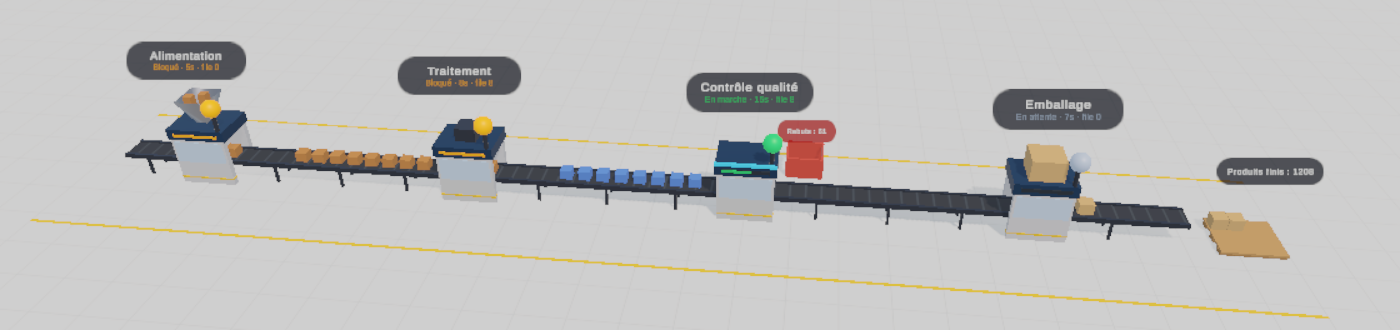
\includegraphics[width=\textwidth]{images/screenshots/vue_globale.png}
\caption{Le jumeau numérique~: accumulation devant le contrôle qualité dans la situation initiale.}
\end{figure}

% ----------------------------------------------------------------- 5. Démo
\section{Démonstration dans le jumeau numérique}
\begin{itemize}[nosep]
  \item \textbf{Avant optimisation}~: visualiser l'accumulation devant le contrôle qualité, le temps d'attente et le débit.
  \item \textbf{Après optimisation}~: appliquer le contrôle à 8~s ou le deuxième poste, observer la diminution de la file.
  \item \textbf{Comparaison}~: afficher les \ac{KPI} avant/après (débit, attente, utilisation des postes, arrêts, rejets), puis l'historique et l'export \ac{CSV}.
\end{itemize}

\end{document}
